\label{sec:methods}
\section{Methods and Materials}

As stated before, two GOFR designs were created and simulated throughout the project. The first design was approached in a bottom-up fashion. This approach allowed for incremental structural changes to the reactor and allowed for the catching of errors in their early stages. Initially, the core size and composition was tested using MCNP criticality tests. After that, various moderating materials (substance that the core was submerged in) were looked at, followed by the material of the enclosing shell. Having finalize the criticality and general internal structure of the reactor, the beam port was added, as well as the FMESH tally, located inside the beam port. The second design was developed as an improvement of the first one, where approximate values of the core and its composition were known, however, geometry of the shell and core itself were adjusted. Although the underlying principles of both designs are similar, the materials used and final results vary significantly.

\subsection{Design 1}

\subsection{Core}

After considering several variations of breeder reactors, all of which were Thorium based, the element of choice for the core was Uranium-235. Due to safety concerns for real-life implementation, its purity could not be 100\%, however criticality calculations were carried at this level out to understand initial core sizes. For reference, anything above 90\% enrichment can be used as a weapon. The size of this pure Uranium core was adjusted multiple times to see the impact of the dimensions on the criticality. These first simulations did not account for a shell reflecting neutrons back into the core, nor did they look at the material inside the shell. The values were vague, however, painted the general picture of how large the core should be and how size impacts the criticality. The next step was to determine how the surrounding material affected the criticality of the core. As seen in table \ref{tab:pure},
water had a better impact on the core's ability to fission than vacuum (results in table \ref{tab:purevac}).

Through these initial simulations, the core was to be surrounded in water for optimum criticality and neutron moderation. The next step was to vary the material of the shell, against which the neutrons would reflect. A thickness of $5cm$ was arbitrarily chosen to make sure the particles would not escape the chamber. Between zirconium and graphite, the latter performed better in reflecting the neutrons and sustaining the nuclear reactions. This was to be expected since zirconium is practically transparent to neutrons. This is seen by results of our simulations in tables \ref{tab:purezrw} and \ref{tab:puregraphitew}.

The final step in the core design was to look at the enrichment percentage. Again, anything above 90\% is considered weapons grade and is extremely dangerous. Low-power reactors usually have enrichment percentages of 3\%-7\%, although some go as high as 20\%. Tables \ref{tab:variations} shows variations between the dimensions of the core and resulting criticalities. The final core design\footnote{For a full list of tables of reactivity values, see the results - section \ref{sec:results}.} was settled to be a cube, side length of $l=30cm$. The U-235 enrichment level would be 15\%, yielding a k-coefficient of $k=1.06625$.

\subsection{Shell}

The surrounding shell and its geometry have several purposes in the reactor:

\begin{enumerate}
	\item Neutron reflection. The neutrons that are emitted from the core need to not be lost after one interaction. As a result, the surrounding shell's geometry was optimized to increase reflectivity of particles back into the core. The thermal neutrons will reflect off of the walls and be directed towards the core to trigger further fissions.
	\item Thermal regulation. Any heat given off by the fission reactions needs to be transported out of the system to control the temperature. This is outside the scope of the project, however, some discussion is given in section \ref{sec:future}.
	\item Particle interaction. This is a middle ground between the previous two purposes. The material that the core is submerged in plays an important role in particle interaction. Materials looked at were water, aluminum, graphite and vacuum.
\end{enumerate}

\subsubsection{Neutron reflection}

An already existing example of reflection was taken into account when looking at the shell's neutron reflection capabilities - a parabolic dish. A ray diagram of how a parabolic reflector works can be seen in figure \ref{fig:parabola}.

\begin{figure}[!htbp]
\caption{Parabolic reflector.}
\label{fig:parabola}
\centering
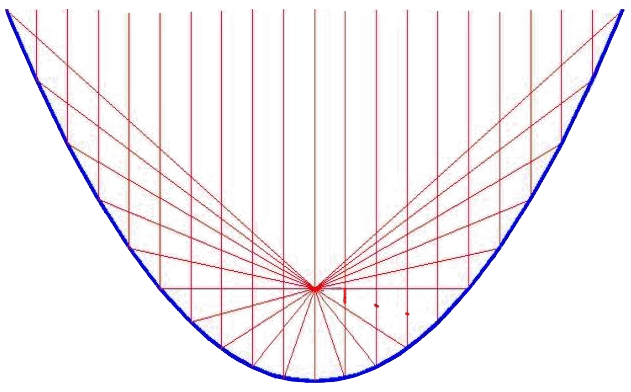
\includegraphics[width=0.75\textwidth]{parabola.png}
\end{figure}

From this, a circular design of the shell was implemented for initial simulations, with the reactor core in the middle. However, looking at the structure presented in figure \ref{fig:structure}, a problem arose when directing neutrons.

\begin{figure}[!htbp]
\caption{Core and shell structures.}
\label{fig:structure}
\centering
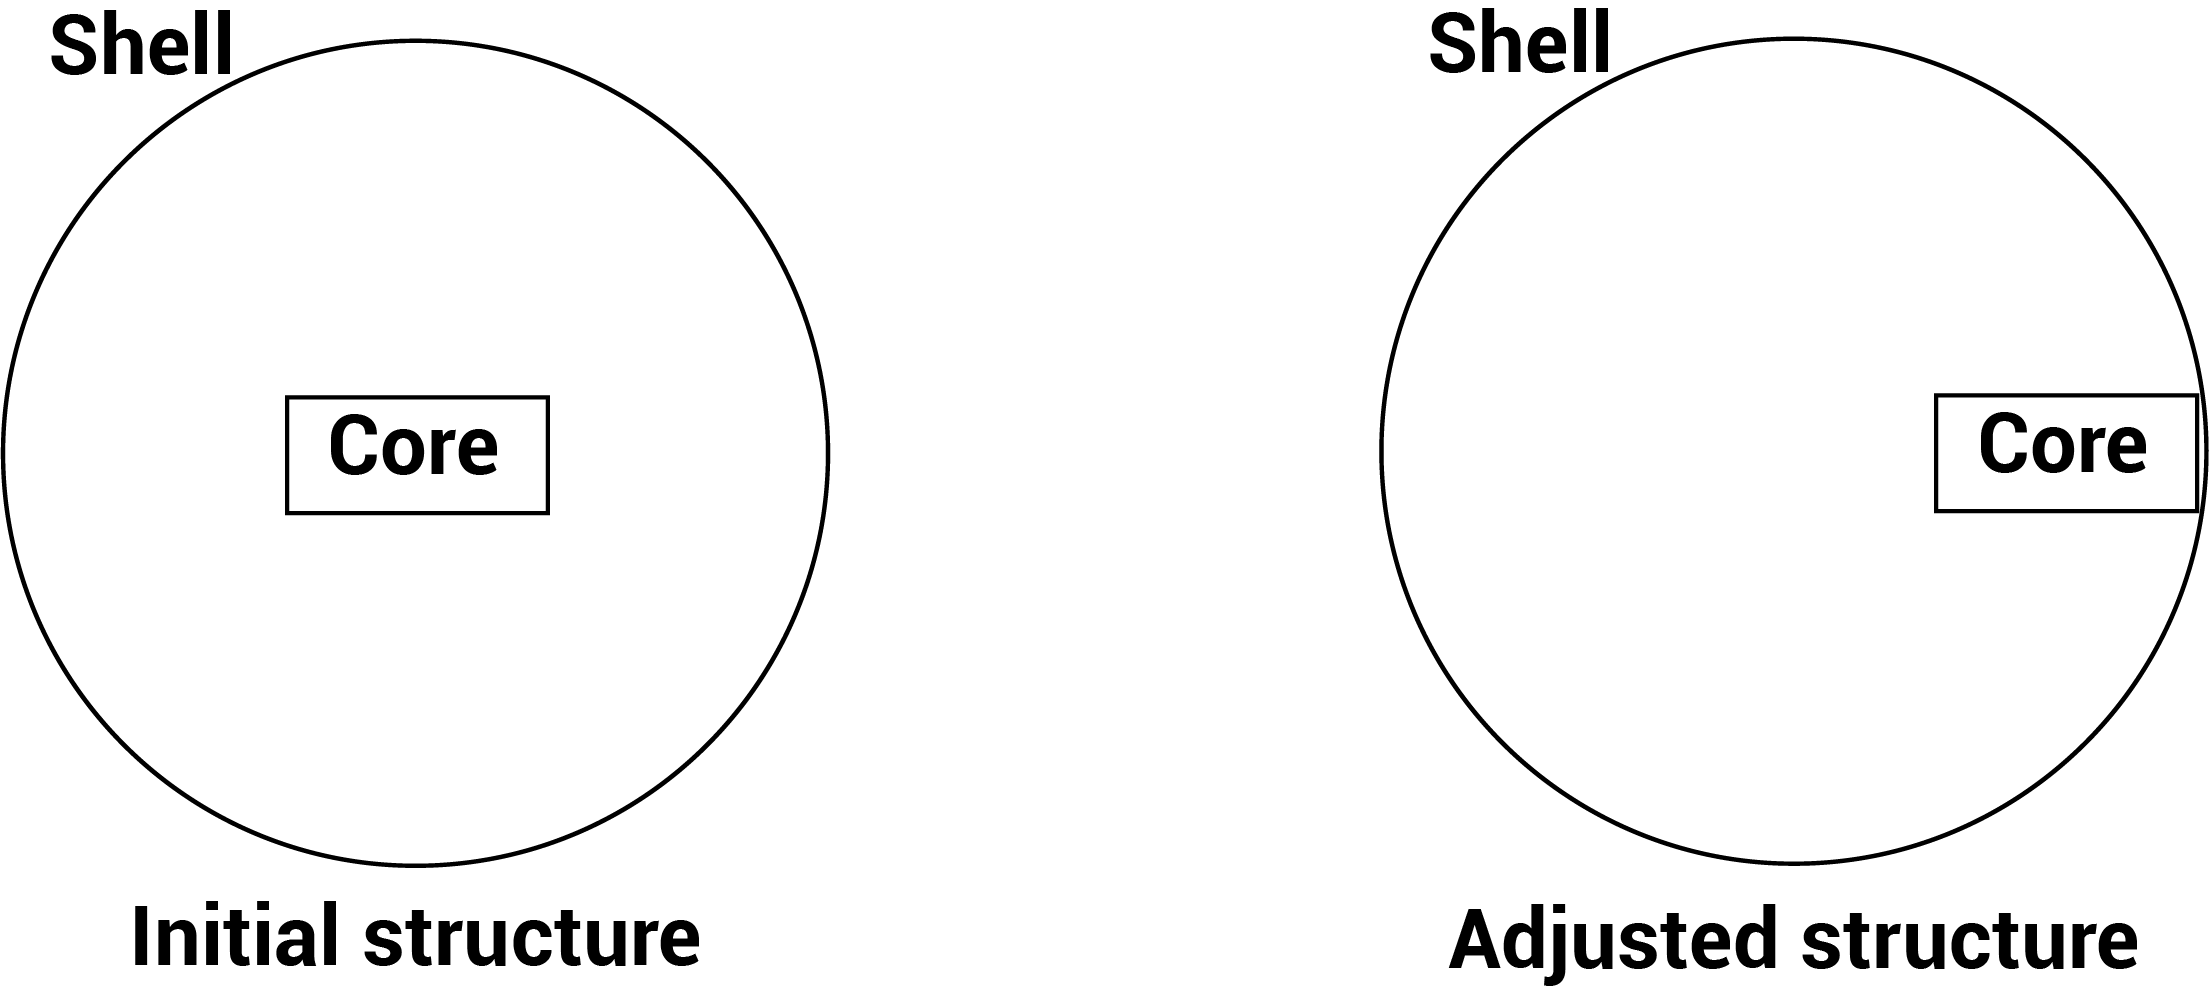
\includegraphics[width=0.75\textwidth]{structure.png}
\end{figure}

Neutrons that are to be used in research would be extremely difficult to direct towards an opening. Whatever added directing structure  would interfere with the parabolic reflective properties. As a result, a decision was made to move the core to one edge of the shell, seen under "Adjusted structure" in figure \ref{fig:structure}.

\subsubsection{Particle interaction}

Several materials were looked at with which to fill the shell around the core. These were water, aluminum, graphite and vacuum. For the first design, water was used for several reasons. Vacuum and graphite would not moderate the neutrons at all, hence failing to help trigger further reactions. Aluminum was not yet looked at in detail due to concerns with thermal dissipation. Alongside this, using water yielded a criticality coefficient of $k=1.06625$, which was ideal for sustaining the fission reactions.

\subsection{Chamber}

With the core shifted to the side of the enclosing shell and all materials chosen, it was now possible to add the neutron chamber, or beam port. One side of the core's structure would be directly exposed to the chamber. As a result, the neutrons produced on that side would be emitted directly for flux calculations and use. The other 5 sides of the rectangular core structure would be fueling the fission reactions through the emission and reflection of thermal neutrons within the shell itself. The cross section of the chamber is 30x30cm in order to capture all particles emitted from one face of the core.

\begin{figure}[!htbp]
\caption{Shell, core, chamber structure.}
\label{fig:chamber}
\centering
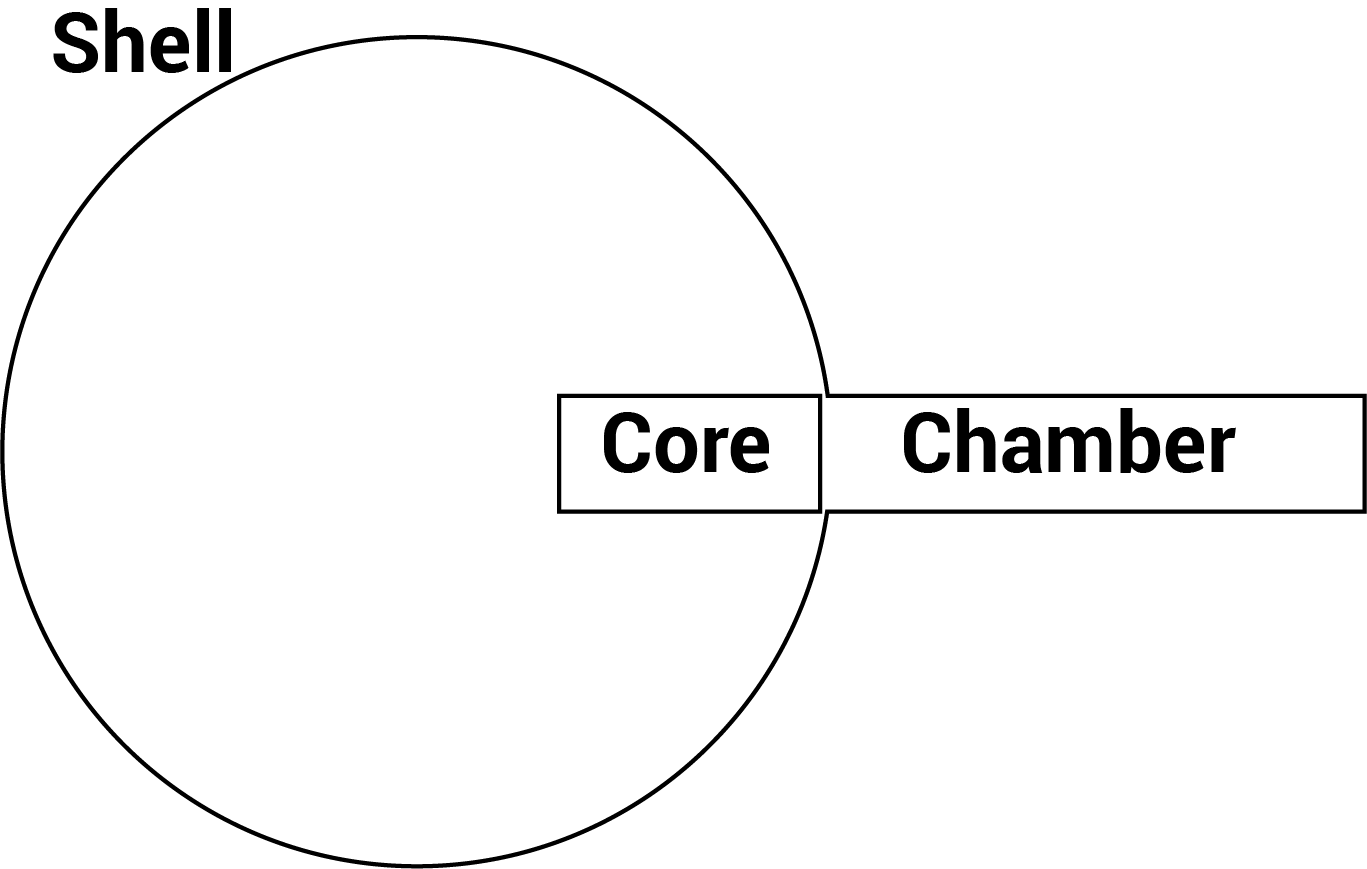
\includegraphics[width=0.75\textwidth]{chamber.png}
\end{figure}

The placement of the core reduces particle leak, however, due to the nature of the geometry (cube placed against a spherical surface), some neutrons may leak back into the shell. The flux lost due to this is negligible since the returned neutrons will fuel further fission reactions after being reflected back into the core by the shell. The structure of the shell, core and neutron chamber can be seen in figure \ref{fig:chamber}. 

\subsection{Tally}

Naturally, the neutron flux tally will be carried out in the chamber. Due to the fact that the primary particles are emitted directly into the beam port, the distance at which the tally is run is not as important in this design as it is in the next. The location was chosen to be 5cm out from the opening of the beam port.

\subsection{Design 2}

The second design stemmed from the first one. Since a general understanding of material compositions and particle behavior was known now (mainly the core size, tally location etc.), these properties were optimized further. Aluminum was looked at as another material to fill the space around the core with. It proved to moderate the neutrons in a better fashion than water. Instead of interacting with them directly and changing their trajectories, they were able to follow their initial courses more often than not. As a result, the optical properties of the reflector were more pertinent here than in the initial design.

Through this, the next adjustment was made - the focal point. An optical reflector has a point where all of the rays are focused into one. This concept was applied to the neutron beams. As a result, the tally was placed as this location - the location of the focal point. Because of this, the maximum flux value was doubled as all of the particles were concentrated into a much smaller area in the tally (as opposed to being sent fairly uniformly through the complete volumetric tally).

In order to fully take advantage of the optical properties, however, overall shell geometry was adjusted as well. Instead of being an actual sphere, the shape resembles an ellipsoid. The rest of the shell's walls converge on the beam port in order to help facilitate the movement of neutrons towards the focal point. Finally, in order to better resemble an isotropic source, the shape of the core was changed to a sphere, with a radius of $r=25cm$. To account for the changes in geometry, the enrichment of the core was increased to 19.9\%. Alongside this, it was alloyed with Zirconium Hydride, $ZrH_4$. Final diagram and example particle paths can be seen in the results - section \ref{sec:results}.

